\section{Task 2}
% Contents:
% - Introduce the problem
% - Explain why total number is not constant, and choices
% - Explain edge conditions
% - Euler method
% Explain different parts of results, impact of parameters

A model for the modelling of sickness over time is the SIR-model. It is given by
\begin{equation}
    \begin{split}
        \frac{dS}{dt} &= -\beta I S \\
        \frac{dI}{dt} &= \beta IS - \gamma I \\
        \frac{dR}{dt} &= \gamma I. \\
    \end{split}
\end{equation}
However, it does not describe the spatial spread of an illness, which can be accommodated for by modifying the equations slightly. We introduce
two dispersion terms to account for the spread in space and obtain the following modified equations
\begin{equation}
    \begin{split}
        \frac{dS}{dt} &= -\beta I S + \mu_S \Delta S \\
        \frac{dI}{dt} &= \beta IS - \gamma I + \mu_I \Delta I\\
        \frac{dR}{dt} &= \gamma I. \\
    \end{split}
\end{equation}
Combined with initial values and boundary conditions, this can be solved with numerical schemes.

\subsection{Numerical scheme}
In the following, we further assume that $S(t) + I(t) + R(t) = 1$, so that we are always working with percentages of the total population instead of the actual population.
We will also just consider the case with two spatial dimensions, and one dimension in time.
To solve the equations we will use the Forward-Euler method, which on these equations results in the following scheme
\begin{equation}
    \begin{split}
        S_{n,m}^{l+1} &= S_{n,m}^l + k(-\beta I_{n,m}^l S_{n,m}^l + \mu_S \Delta_h S_{n,m}^l) \\
        I_{n,m}^{l+1} &= I_{n,m}^l + k(\beta I_{n,m}^l S_{n,m}^l - \gamma I_{n,m}^l +  \mu_I \Delta_h I_{n,m}^l) \\
        R_{n,m}^{l+1} &= R_{n,m}^l + k \gamma I_{n,m}^l,  \\
    \end{split}
\end{equation}
where
\begin{equation*}
    \Delta_h X_{n,m}^l = \frac{1}{h^2}(X_{n+1, m}^l + X_{n-1, m}^l + X_{n, m+1}^l + X_{n, m-1}^l - 4X_{n,m}^l).
\end{equation*}
Here $k$ is the timestep in the time domain, and $h$ the timestep in the two spatial domains. That means the we operate with the same timestep in both the spatial dimensions.
$X_{n,m}^l$ corresponds to the numerical solution at $(x_n,y_m,t_l)$, where $X\in \{S,I,R\}$. It should be noted that the Forward-Euler scheme is
not stable for all combinations of $h$ and $k$. In the a little bit simpler equation $\frac{\partial u}{\partial t} = \alpha \Delta u$, it is stable for all $(h,k)$
such that $\frac{\alpha k}{h^2} < \frac{1}{4}$. This gives a rough estimate for when it is stable in our scheme as well.

Additionally we need both initial values and boundary conditions to be able to solve the problem numerically.
The initial values describes the initial distributions of susceptible, infected and recovered people, while
the boundary conditions describe how the different people move over the problem border. Since we want the population to be constant and closed, that is no people arrive or leave
the area, we set the boundary conditions to be
\begin{equation}
    \begin{split}
        \nabla S(\Omega) &= \Vec{0} \\
        \nabla I(\Omega) &= \Vec{0} \\
        \nabla R(\Omega) &= \Vec{0}, \\
    \end{split}
\end{equation}
where $\Omega$ is the edge of the domain. In discretized form this reads
\begin{equation}
    \begin{split}
        \frac{\Delta_h X_{n,m}^l - \nabla_h X_{n,m}^l}{2h} = 0,
    \end{split}
\end{equation}
or equivalently
\begin{equation}
    \begin{split}
        X_{n,-1}^l &= X_{n, 1}^l \\
        X_{n,N+2}^l &= X_{n, N}^l \\
        X_{-1,m}^l &= X_{1, m}^l \\
        X_{N+2,m}^l &= X_{N, m}^l \\
        & n,m \in [1, N]
    \end{split}
\end{equation}


\subsection{Results}
Although the conditions are set to enforce constant population size, we will still observe errors in the numerical scheme. A possible solution of this problem is to not 
solve for $R(t)$ explicitly, but rather to let $R(t)$ be the remains
\begin{itemize}
    \item Let $R$ be the "rest" of the population without solving the actual equation. $\implies$ The total number of people is stable at $1$, but the number of recovered people is not accurate.
    \item Solve the $R$ equation as stated, and accept that the population number is not fixed at 1, although it should not deviate far from 1.
\end{itemize}
Ideally both solutions would give the same answer.
In our solution we have done the latter.

\begin{figure}
    \centering
    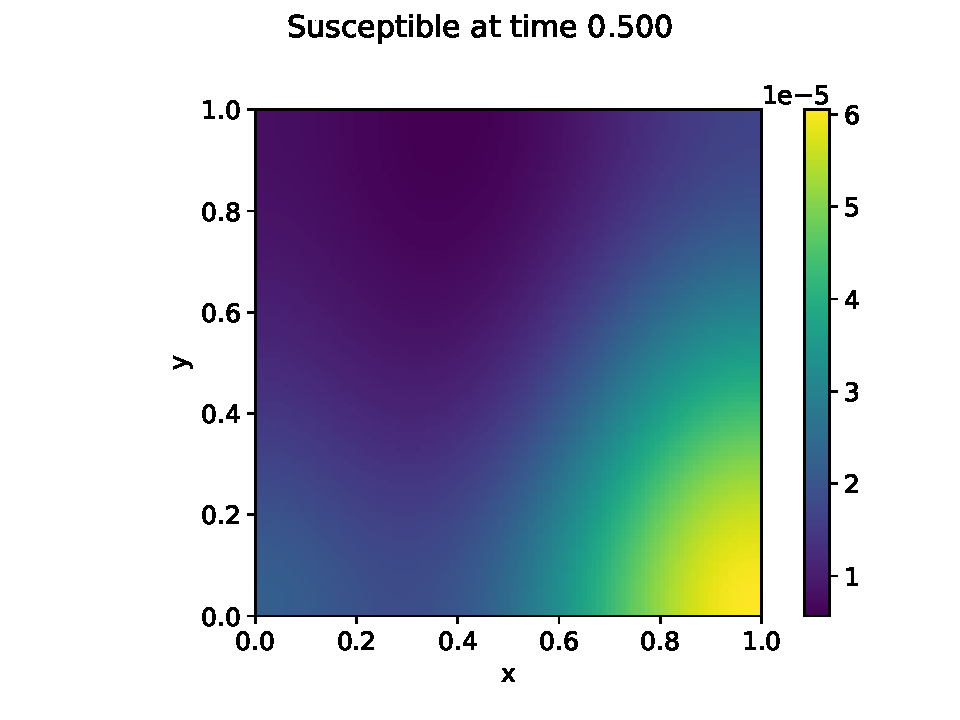
\includegraphics[width=\textwidth]{report/Images/plots/plot-i_t=5000-0.pdf}
    \caption{Caption}
    \label{fig:enter-label}
\end{figure}

(plot from one square over time)

(plot of population deviation from 1)

The size of the domain influences the parameter choices. The larger domain, the larger the step size in that domain in order to get the same runtime, but that includes larger errors.
In addition the small stepsize, the larger the constants such as $\beta$ needs to be in order to get the same results.


% TODOS: forskjeller i befolkningstetthet, endringer i beta